\chapter{Lecture 31 - Solving BVPs with the Finite Difference Method}
\label{ch:lec31n}
\section{Objectives}
The objectives of this lecture are to:
\begin{itemize}
\item Describe the Finite Difference Method (FDM) for BVPs.
\item Demonstrate the method with an example problem.
\end{itemize}
\setcounter{lstannotation}{0}

\section{Finite Difference Method for Boundary Value Problems}

In the Finite Difference Method, the derivatives in the differential equation are replaced with \emph{finite difference approximations.}  The domain is divided into finite intervals defined by grid points as shown in Figure \ref{fig:lec31-fd-schematic}
\begin{figure}[h!]
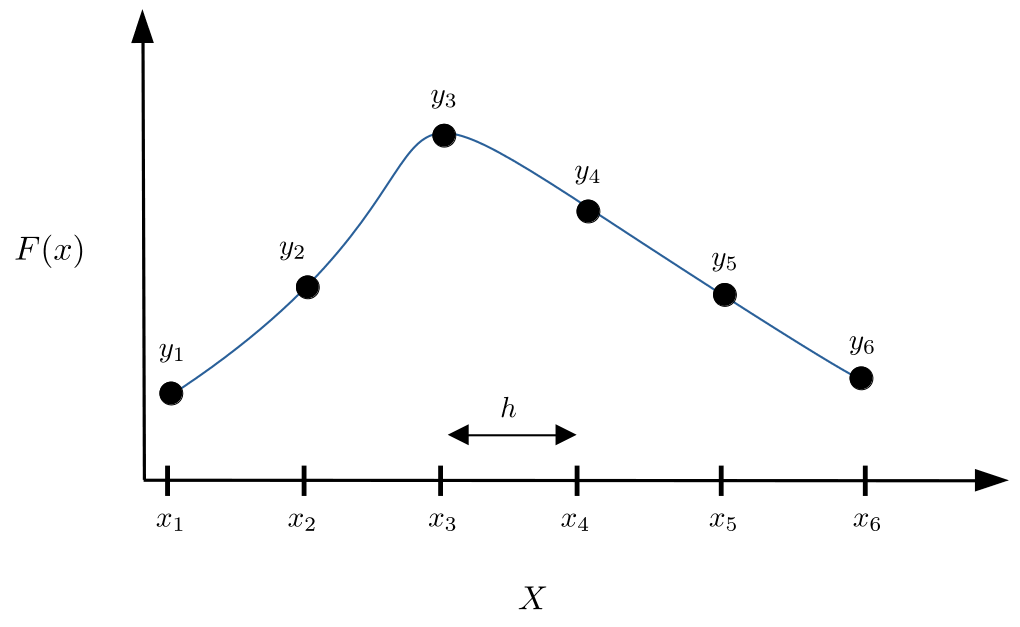
\includegraphics{lec31n-fd-schematic.png}
\caption{Function discretized into a finite number of intervals for the FDM.}
\label{fig:lec31-fd-schematic}
\end{figure}
The solution is approximated by the value of the dependent variable at each grid point.  

\vspace{1.0cm}

\noindent Consider the linear boundary value problem:

\begin{table}
\begin{tabular}{l l}
Govering Equation: & $y^{\prime \prime} + f(x)y^{\prime} + g(x)y = P(x), \ \ a < x < b$ \\
BCs: & $y(a) = Y_a, \ \ y(b) = Y_b$ \\
\end{tabular}
\end{table}

\vspace{0.25cm}

\noindent We will apply finite difference formulas with $\mathcal{O}(h^2)$ convergence for each grid point.  As a reminder, finite difference formulas with this property are shown in Table \ref{tab:lec31n-fd-formulas-yp} and Table \ref{tab:lec31n-fd-formulas-ypp}.

\begin{margintable}
\begin{tabular}{l | c}
\hline
Grid Point & $y^{\prime}$ \\ \hline
left boundary & $\frac{-3y_i + 4y_{i+1} - y_{i+1}}{2h}$ \\ \hline 
interior point & $\frac{y_{i+1}-y_{i-1}}{2h} $ \\ \hline
right boundary & $\frac{y_{i-2}-4y_{i-1}+3y_i}{2h}$ \\ \hline
\end{tabular}
\caption{Finite difference formulas for $y^{\prime}$ with $\mathcal{O}(h^2)$ convergence.}
\label{tab:lec31n-fd-formulas-yp}
\end{margintable}

\begin{margintable}
\begin{tabular}{l | c}
\hline
Grid Point & $y^{\prime \prime}$ \\ \hline
left boundary & $\frac{2y_i-5y_{i+1}+4y_{i+1}-y_{i+3}}{h^2}$ \\ \hline 
interior point & $\frac{y_{i-1}-2y_i+y_{i+1}}{h^2} $ \\ \hline
right boundary & $\frac{-y_{i-3}+4y_{i-2}-5y_{i-1}+2y_i}{h^2}$ \\ \hline
\end{tabular}
\caption{Finite difference formulas for $y^{\prime \prime}$ with $\mathcal{O}(h^2)$ convergence.}
\label{tab:lec31n-fd-formulas-ypp}
\end{margintable}

\newthought{Consider each term} of the governing equation.  We will apply the appropriate finite difference formulas to create a linear system of equations.

\begin{enumerate}
\item First term:
\begin{equation*}
y^{\prime \prime} \approx
\underbrace{
\frac{1}{h^2}
\bracketMatrixstack{
2 & -5 & 4 & -1 & 0 & 0 \\
1 & -2 & 1 & 0 & 0 & 0 \\
0 & 1 & -2 & 1 & 0 & 0 \\
0 & 0& 1 & -2 & 1 & 0 \\
0 & 0 & 0 & 1 & -2 & 1 \\
0 & 0 & -1 & 4 & -5 & 2
}}_{\text{D}_{\text{xx}}}
\underbrace{
\bracketVectorstack{
y_1 \\
y_2 \\
y_3 \\
y_4 \\
y_5 \\
y_6
}}_{y}
\end{equation*}

\item Second term:
\begin{equation*}
f(x)y^{\prime} \approx
\underbrace{
\bracketMatrixstack{
f(x_1) & 0 & 0 & 0 & 0 & 0 \\
0 & f(x_2) & 0 & 0 & 0 & 0 \\
0 & 0 & f(x_3) & 0 & 0 & 0 \\
0 & 0 & 0 & f(x_4) & 0 & 0 \\
0 & 0 & 0 & 0 & f(x_5) & 0 \\
0 & 0 & 0 & 0 & 0 & f(x_6)
}}_{F}
\underbrace{
\frac{1}{2h}
\bracketMatrixstack{
-3 & 4 & -1 & 0 & 0 & 0 \\
-1 & 0 & 1 & 0 & 0 & 0 \\
0 & -1 & 0 & 1 & 0 & 0 \\
0 & 0 & -1 & 0 & 1 & 0 \\
0 & 0 & 0 & -1 & 0 & 1 \\
0 & 0 & 0 & 1 & -4 & 3
}}_{\text{D}_{\text{x}}}
\bracketVectorstack{
y_1 \\
y_2 \\
y_3 \\
y_4 \\
y_5 \\
y_6
}
\end{equation*}

\item Third term:
\begin{equation*}
g(x)y \approx
\underbrace{
\bracketMatrixstack{
g(x_1) & 0 & 0 & 0 & 0 & 0 \\
0 & g(x_2) & 0 & 0 & 0 & 0 \\
0 & 0 & g(x_3) & 0 & 0 & 0 \\
0 & 0 & 0 & g(x_4) & 0 & 0 \\
0 & 0 & 0 & 0 & g(x_5) & 0 \\
0 & 0 & 0 & 0 & 0 & g(x_6)
}}_{G}
\bracketVectorstack{
y_1 \\
y_2 \\
y_3 \\
y_4 \\
y_5 \\
y_6
}
\end{equation*}
\item Right-hand Side:
\begin{equation*}
p(x) \approx
\underbrace{
\bracketVectorstack{
p(x_1) \\
p(x_2) \\
p(x_3) \\
p(x_4) \\
p(x_5) \\
p(x_6)
}}_{P}
\end{equation*}
\end{enumerate}

\noindent Using the notation shown above, we can combine all of the terms into a linear system of equations:
\begin{align*}
y^{\prime \prime}+f(x)y^{\prime} + g(x)y &= p(x) \\
D_{xx}y + FD_xy + Gy &= P \\
\left[D_{xx} + FD_x + G\right]y &= P \\
Ly &= P
\end{align*}

\newthought{This linear system} of equations is a discrete representation of the differential equation.  In order to find a unique solution to the boundary value problem, we must apply the boundary conditions.

\subsection{Dirichlet Boundary Conditions}
For this course, we will only consider Dirichlet (type-1) boundary conditions for problems that we solve with the finite difference method.  For this type of a boundary condition, our goal is to force the finite difference solution to be equal to the prescribed value at the boundaries.  One simple way to do this is, as follows:
\begin{enumerate}
\item Replace the first row of $L$ with all zeros except the first entry, which you will set to $L(1,1)=1$.  
\item Replace the first entry on the right-hand side to $Y_a$. 
\item Replace the last row of $L$ with all zeros except the last entry, which you will set to $L(n,n) = 1$, where $n$ is the number of equations in your system.\sidenote{Of course, the number of equations, $n$, is equal to the number of grid points in your discrete representation of $y(x)$.}
\item Replace the last entry on the right-hand side to $Y_b$.
\end{enumerate}
The resulting system of equations is illustrated schematically in Figure \ref{fig:lec31n-fd-bc}.
\begin{marginfigure}
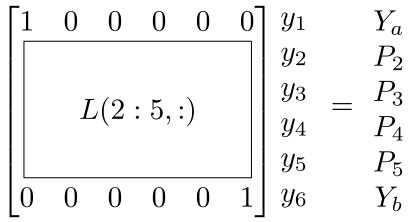
\includegraphics{lec31n-fd-bc.png}
\caption{Linear system after applying Dirichlet boundary conditions.}
\label{fig:lec31n-fd-bc}
\end{marginfigure}

\subsection{Solving the System of Equations}
Since this is a linear system of equations, readers who have been following the book from the beginning should immediately know that the answer is either:
\begin{enumerate}
\item A direct method like Gauss elimination, LU decomposition, or whatever method \lstinline[style=myMatlab]{mldivide} chooses if you are working in a MATLAB environment and have MATLAB built-in solvers available to you.
\item An iterative method like Jacobi, Gauss-Seidel, successive-overrelaxation or MATLAB built-in methods like \lstinline[style=myMatlab]{pcg}, or \lstinline[style=myMatlab]{gmres}
\end{enumerate}
Two key points that may influence your decision, that I want to highlight now are as follows:

\begin{enumerate}
\item \emph{Most of the entries of $L$ are zero}.  For this small system, it may not be as obvious. If we instead discretized the domain into, for example, 10,000 grid points, the structure of the matrices would be the same.  Namely that, while each row would now have a total of 10,000 entries, only 3 or 4 of the entries in each row would be non-zero.  If high accuracy is demanded users may be motivated to use $10^5$ or $10^6$ grid points.  In such cases it is essential that sparse matrix data structures are used and algorithms that avoid fill-in are chosen for the solution process.\sidenote{Of course, for this example we have chosen finite difference formulas with $\mathcal{O}(h^2)$ convergence.  If we had chosen formulas with higher-order convergence behavior, the sparsity of $L$ would be reduced but, except in cases where high-order spectral methods are used (not discussed in this class), the matrix $L$ remains sparse.}

\item \emph{The matrix $L$ is nearly symmetric}.  Indeed, alternative methods for applying Dirichlet boundary conditions have been devised specifically to preserve symmetry of the linear system of equations.  In this case, direct algorithms like \lstinline[style=myMatlab]{chol} or iterative methods like \lstinline[style=myMatlab]{pcg} that are designed for symmetric matrices may be used and generally result in obtaining a solution with less computational work.  
\end{enumerate}

\subsection{Constructing Sparse Differentiation Matrices}
Before we move along to example problems, we will present functions that we will use to construct the 1\textsuperscript{st}- and 2\textsuperscript{nd}-order differentiation matrices.  We will take advantage of MATLAB's tools for constructing sparse matrices.

A MATLAB function for constructing the 1\textsuperscript{st}-order differentiation matrix is shown in the listing below:
\marginnote[6.0cm]{

\vspace{1.0cm}

\noindent\ref{lst:ann31n-diff-mat-1} Per MATLAB style guides we pre-allocate space to store non-zero matrix element data.  If $N$ is large, this is much more efficient than having MATLAB ``grow'' the data vectors as we go.   

\vspace{8.0cm}

\noindent\ref{lst:ann31n-diff-mat-2} See the MATLAB documentation for the sparse matrix constructor: \lstinline[style=myMatlab]{sparse}.  
}
\begin{lstlisting}[style=myMatlab,name=lec31n-yp-mat]
function dx_sp = Dx(a,b,N)
% function dx_sp = Dx(a,b,N) returns a sparse matrix
% for a first order differentiation matrix using 2nd-order
% centered-difference for interior nodes and 2nd-order
% forward/backward-difference nodes for the respective 
% endpoints of the domain.
%
% Inputs:
% a - scalar, left endpoint of domain
% b - scalar, right endpoint of domain
% N - number of points in the domain inclusive of the endpoints

% compute the number of entries in the sparse matrix:
% 3-each for the 2 endpoints + 2 each for the N-2 interior points
NumEntries = 3*2 + 2*(N-2);

% Initialize the sparse matrix data vectors
dx_row = nan(NumEntries,1); /*!\annotation{lst:ann31n-diff-mat-1}!*/
dx_col = nan(NumEntries,1);
dx_val = nan(NumEntries,1);

h = (b-a)/(N-1);

% first three entries for the left end-point
dx_row(1) = 1; dx_col(1) = 1; dx_val(1) = -3/(2*h);
dx_row(2) = 1; dx_col(2) = 2; dx_val(2) = 4/(2*h);
dx_row(3) = 1; dx_col(3) = 3; dx_val(3) = -1/(2*h);

ind = 4;

for i = 2:(N-1)
   dx_row(ind) = i; dx_col(ind) = i-1; dx_val(ind) = -1/(2*h);
   ind = ind+1;
   dx_row(ind) = i; dx_col(ind) = i+1; dx_val(ind) = 1/(2*h);
   ind = ind+1;   
    
end

% last three entries for the right end-point
dx_row(ind) = N; dx_col(ind) = N; dx_val(ind) = 3/(2*h);
ind = ind+1;
dx_row(ind) = N; dx_col(ind) = N-1; dx_val(ind) = -4/(2*h);
ind = ind+1;
dx_row(ind) = N; dx_col(ind) = N-2; dx_val(ind) = 1/(2*h);

dx_sp = sparse(dx_row,dx_col,dx_val,N,N); /*!\annotation{lst:ann31n-diff-mat-2}!*/

end
\end{lstlisting}

\newthought{The function to} construct a 2\textsuperscript{nd}-order differentiation matrix is similar and shown in the listing below:
\begin{lstlisting}[style=myMatlab,name=lec31-ypp-mat]
function dxx_sp = Dxx(a,b,N)
% function dxx_sp = Dxx(a,b,N) returns a sparse matrix
% for a second order differentiation matrix using 2nd-order
% centered-difference for interior nodes and 2nd-order
% forward/backward-difference nodes for the respective 
% endpoints of the domain.
%
% Inputs:
% a - scalar, left endpoint of domain
% b - scalar, right endpoint of domain
% N - number of points in the domain inclusive of the endpoints

% compute the number of entries in the sparse matrix:
% 4-each for the 2 endpoints + 3 each for the N-2 interior points
NumEntries = 4*2 + 3*(N-2);

% Initialize the sparse matrix data vectors
dx_row = nan(NumEntries,1);
dx_col = nan(NumEntries,1);
dx_val = nan(NumEntries,1);

h = (b-a)/(N-1);

% first three entries for the left end-point
dx_row(1) = 1; dx_col(1) = 1; dx_val(1) = 2/(h^2);
dx_row(2) = 1; dx_col(2) = 2; dx_val(2) = -5/(h^2);
dx_row(3) = 1; dx_col(3) = 3; dx_val(3) = 4/(h^2);
dx_row(4) = 1; dx_col(4) = 4; dx_val(4) = -1/(h^2);

ind = 5;

for i = 2:(N-1)
   dx_row(ind) = i; dx_col(ind) = i-1; dx_val(ind) = 1/(h^2);
   ind = ind+1;
   dx_row(ind) = i; dx_col(ind) = i; dx_val(ind) = -2/(h^2);
   ind = ind+1;
   dx_row(ind) = i; dx_col(ind) = i+1; dx_val(ind) = 1/(h^2);
   ind = ind+1;   
    
end

% last four entries for the right end-point
dx_row(ind) = N; dx_col(ind) = N; dx_val(ind) = 2/(h^2);
ind = ind+1;
dx_row(ind) = N; dx_col(ind) = N-1; dx_val(ind) = -5/(h^2);
ind = ind+1;
dx_row(ind) = N; dx_col(ind) = N-2; dx_val(ind) = 4/(h^2);
ind = ind+1;
dx_row(ind) = N; dx_col(ind) = N-3; dx_val(ind) = -1/(h^2);

dxx_sp = sparse(dx_row,dx_col,dx_val,N,N);

end
\end{lstlisting}

\subsection{Example \#1}

Consider the following boundary value problem:

\begin{table}
\begin{tabular}{l l}
Govering Equation: & $y^{\prime \prime} -4y = 0, \ \ 0 < x < 1$ \\
BCs: & $y(0) = 0, \ \ y(1) = 5$ \\
\end{tabular}
\end{table}

\vspace{0.25cm}

\noindent The analytic solution to this BVP is: $y(x) = 5\sinh{(2x)}/\sinh{(2)}$.  In the listing below we present the MATLAB code to find an approximate solution using the finite difference method.

\setcounter{lstannotation}{0}

\marginnote[3.0cm]{

\vspace{2.2cm}

\noindent\ref{lst:ann31n-ex-1} The constructor \lstinline[style=myMatlab]{speye(N,N)} creates a sparse $N \times N$ identity matrix.

}
\begin{lstlisting}[style=myMatlab,name=lec31n-ex1]
clear
clc
close 'all'

a = 0; b = 1;
N = 200;
x = linspace(a,b,N); x = x';

% known exact solution
y_exact = @(x) 5*sinh(2*x)./sinh(2);

Dxx_op = Dxx(a,b,N); % get 2nd order differentiation matrix
L = Dxx_op - 4*speye(N,N);% form the differential operator /*!\annotation{lst:ann31n-ex-1}!*/
rhs = zeros(N,1); % initialize the right hand side

% apply boundary conditions
L(1,:) = 0; L(1,1) = 1; rhs(1) = 0; 
L(N,:) = 0; L(N,N) = 1; rhs(N) = 5;

y = L\rhs; % solve the system of equations

figure(1)
subplot(2,1,1)
xs = x(1:10:end);
plot(xs,y_exact(xs),'sr',...
    x,y,'-c','linewidth',3);
ylabel('Numeric Solution','fontweight','bold');
title('Solution to: y^{\prime\prime} - 4y = 0;  y(0)=0; y(1)=5','fontsize',14);
set(gca,'fontweight','bold');
legend('Exact','Numeric','location','northwest');
grid on

subplot(2,1,2)
plot(x,abs(y - y_exact(x)),'-r','linewidth',3);
ylabel('Numerical Error','fontweight','bold')
set(gca,'fontweight','bold');
grid on
\end{lstlisting}
\begin{marginfigure}[-10.0cm]
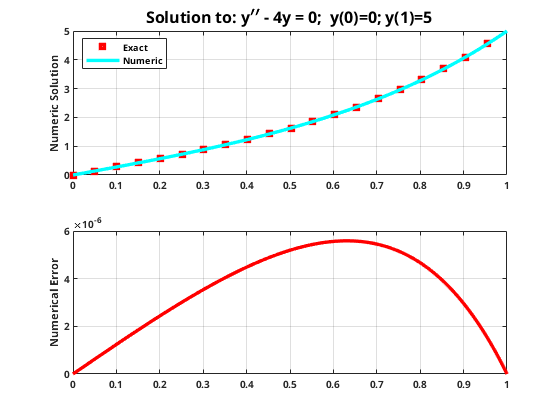
\includegraphics{lec31n-ex1-sol.png}
\caption{Finite difference method solution to Example \#1 and point-wise error. N = 200}
\label{fig:lec31n-ex1-sol}
\end{marginfigure}

\begin{marginfigure}[-2.0cm]
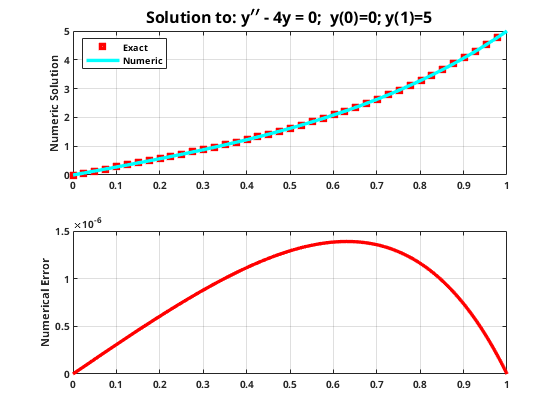
\includegraphics{lec31n-ex1-sol2.png}
\caption{Finite difference method solution to Example \#1 and point-wise error. N = 400}
\label{fig:lec31n-ex1-sol2}
\end{marginfigure}
The solution and error are shown in Figure \ref{fig:lec31n-ex1-sol}. Note that the error is (as expected?) zero at the boundaries since the boundary conditions are applied exactly at those locations.  If we double the number of grid points, by what factor do we expect the solution to improve?  Figure \ref{fig:lec31n-ex1-sol2} shows that the maximum error is reduced by a factor of 4 which is what one should expect for a 2\textsuperscript{nd}-order convergent approximation.   


\subsection{Example \#2}
As a somewhat more difficult example, consider the boundary value problem below:

\begin{table}
\begin{tabular}{l l}
Govering Equation: & $x^2y^{\prime \prime} - 3xy^{\prime} + 3y = 0, \ \ 1 < x < 2$ \\
BCs: & $y(1) = 0, \ \ y(2) = 0$ \\
\end{tabular}
\end{table}

\vspace{0.25cm}

\noindent The exact solution is: $y(x) = 12x-15x^3 + 3x^5$.\marginnote{\textbf{Note:} This result was arrived at using the (very handy) method of \emph{``manufactured solutions.''} This is where you devise of a solution first, $y_s(x)$, then plug it into the differential operator, $L(y_s)$.  The result, $L(y_s)=p(x)$ becomes the source term and you evaluate $y_s$ at the boundaries to get the Dirichlet boundary conditions.  This is a well-accepted technique for validating your solver.}

The MATLAB code to solve this equation is presented in the listing below:
\marginnote{

\vspace{2.0cm}

\noindent \ref{lst:ann31n-ex-2} Compare these lines of code to the governing equation.  Does the syntax make sense? As an example, the nested functions \lstinline[style=myMatlab]{sparse(diag(x.^2))}, where \lstinline[style=myMatlab]{x} is a vector, results in a diagonal matrix with the values of $x^2$ along the diagonal stored in a sparse matrix representation.

}
\begin{lstlisting}[style=myMatlab,name=lec31n-ex2]
a = 1; b = 2;
N = 100;

Dxx_op = Dxx(a,b,N);
Dx_op = Dx(a,b,N);

x = linspace(a,b,N); x = x';

% known exact solution
y_exact = @(x) 12*x - 15*(x.^3) + 3*(x.^5);

L = (sparse(diag(x.^2)))*Dxx_op - ...
    3*sparse(diag(x))*Dx_op + ...     /*!\annotation{lst:ann31n-ex-2}!*/
    3*speye(N,N);
rhs = 24*(x.^5);

% apply BCs
L(1,:) = 0; L(1,1) = 1; rhs(1) = 0;
L(N,:) = 0; L(N,N) = 1; rhs(N) = 0;

% solve the system
y = L\rhs;

figure(1)
subplot(2,1,1)
xs = x(1:10:end);
plot(xs,y_exact(xs),'sr',...
    x,y,'-c','linewidth',3);
title('Solution to: x^2y^{\prime\prime} - 3xy^{\prime}+3y=24x^5;  y(1)=y(2)=0',...
    'fontweight','bold','fontsize',14);
ylabel('Numeric Solution','fontweight','bold');
set(gca,'fontweight','bold');
legend('Exact','Numeric');
grid on

subplot(2,1,2)
plot(x,abs(y - y_exact(x)),'-r','linewidth',3);
ylabel('Numerical Error')
set(gca,'fontweight','bold');
grid on
\end{lstlisting}
\begin{marginfigure}[-4.0cm]
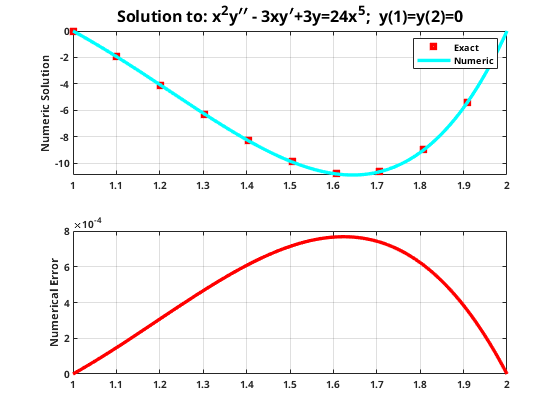
\includegraphics{lec31n-ex2-sol.png}
\caption{Finite difference method solution to Example \#2 and point-wise error.}
\label{fig:lec31n-ex2-sol}
\end{marginfigure}
The solution and error are shown in Figure \ref{fig:lec31n-ex2-sol}.  Readers are encouraged to run this example and confirm 2\textsuperscript{nd}-order convergence to the solution.

